\chapter{Metodología y fases del producto}
\label{metodologia}
\section{Metodología}
La metodología llevada a cabo durante el proyecto es una creación propia basada en caraterísticas
copiadas de metodologías ágiles como el \textbf{'Scrum'} y adaptadas a la forma de trabajar propia.
La idea es estructurar todo el proyecto en diversas iteraciones y durante estas marcarse
objetivos y/o tareas con el fin de añadir funcionalidades completas.

El uso de \textbf{iteraciones} para dividir la carga de trabajo y agrupar tareas nos ayudará
a conseguir acotar la duración de algunas tareas y marcarnos objetivos a corto/medio
plazo. Además de separar por funciones el proyecto, las tareas que conllevan su desarrollo
también deberemos analizarlas e intentar reducir su tamaño y carga lo máximo posible, esto
permite obtener una sensación de éxito de forma rápida lo cual ayuda a mantener una moral y 
motivación altas.

Para poner un ejemplo de como elaborar esta separación por subtareas, el objetivo que vamos a
usar es ``dibujar elementos por pantalla''. Como estamos en un proyecto básado en \ac{ECS} rápidamente
vemos que vamos a requerir mínimo un componente de dibujado \textit{(RenderCmp)} y un 
``RenderSystem'' el cual se encargará de recoger todos los elementos visuales y hacer las
llamadas necesarias para dibujarlos. \\
En caso de no tener una librería de dibujado, otra tarea podría ser el buscar una que sea capaz
de realizar el trabajo requerio y/o implementar una propia
\footnote{Esto supondría una serie de tareas en base a la cantidad de funcionalidades que se requieran.}. 

Para ayudar a la planificación del trabajo usaremos la herramienta `Trello'
~\ref{fig:logos} \footnote{Página de `Trello': https://trello.com/es}
la cual nos permitirá crear diversas listas según el ámbito o el estado de
desarrollo de las distintas tareas que contendrán, cada tarea se ve representada con
una tarjeta la cual puede tener una serie de subtareas asociadas dentro. Esto nos
permitirá tener un registro de todas las labores que quedan por hacer en cada iteración y
cuales ya estan termiandas completamente, además podremos conservar las listas de las tareas
realizadas en iteraciones anteriores para futuras revisiones.

Otra herramienta de control que usaremos durante el desarrollo será `Toggl'
~\ref{fig:logos} \footnote{Página de `Toggl': https://toggl.com}
la cual nos permitirá llevar a cabo un registro de las horas que dedicamos en cada tarea
y agrupar tareas en función del campo de estudio o parte del desarrollor al que pertecen.

\begin{figure}[ht]
\centering
\begin{minipage}[c]{0.45\linewidth}
	\hspace{1cm}
	
\includegraphics[width=0.7\textwidth]{imagenes/metodologia/logo-trello.png}
\end{minipage}
\begin{minipage}[c]{0.45\linewidth}
	
\includegraphics[width=0.7\textwidth]{imagenes/metodologia/logo-toggl.png}
\end{minipage}	
\caption{Logos de Trello y Toggl.}
\label{fig:logos}
\end{figure}

\section{Iteraciones}
En esta sección se comentarán brevemente los objetivos planteados y las tareas que
se han llevado a cabo en cada iteración adjuntando el tablero de `Trello' asociado.

\subsection{Iteración 0}
Esta iteración tenía como proposito terminar de definir la idea para el
proyecto, ya que, todavía era un poco difusa la imagen del producto final que se quería desarrollar.
Para ir entrando en una dinámica productiva e ir definiendo lo que se quería hacer,
comenzamos por iniciar el desarrollo de un propotipo a la vez que preparabamos un poco
los materiales relacionados con la memoria, como puede ser la lectura de las directrices
y/o la revisión de la plantilla de \LaTeX~\ref{img:it_0}.

Al final de esta iteración el prototipo contaba con una versión básica del bucle principal
del juego donde creamos una serie de sistemas, \textit{managers} y entidades además del dibujado
y movimiento\footnote{En esta versión nos limitamos a un ``Goto'' a través de 4 puntos.} de 
estas.

\begin{figure}[ht]
\centering
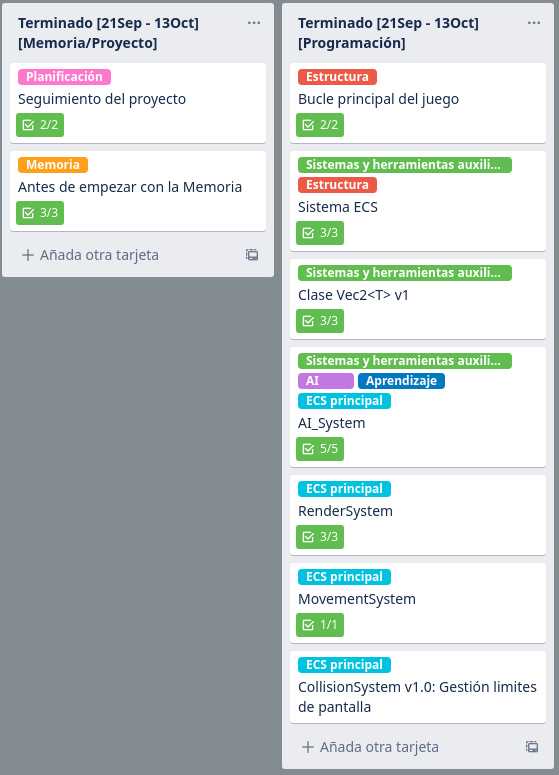
\includegraphics[width=0.45\textwidth]{imagenes/metodologia/tareas_it0.png}
\caption{Lista de tareas realizadas en la iteración 0}
\label{img:it_0}
\end{figure}

\subsection{Iteración 1}
A lo largo de esta iteración seguimos añadiendo sistemas al prototipo como puede ser el
de \textit{Input} el cual nos permitirá interactuar con el producto, además de herramietas
como el mapeado del teclado o el tipo de dato en coma fija en el cual profundizaremos más tarde.

Por otro lado, se comenzó a trabajar en la \ac{IA} del juego creando los primeros comportamientos
y herramientas para cambiar entre ello. Como veremos más adelante también, aquí caeremos en los primeros
errores de concepto a la hora de trabajar con los \textit{`Steering behaviors'}.

Por último, finalizamos la introducción en el uso de \LaTeX, \textit{`JabRef'} y la plantilla comenzando 
así con la redacción de esta memoria~\ref{img:it_1}.

\begin{figure}[ht]
\centering
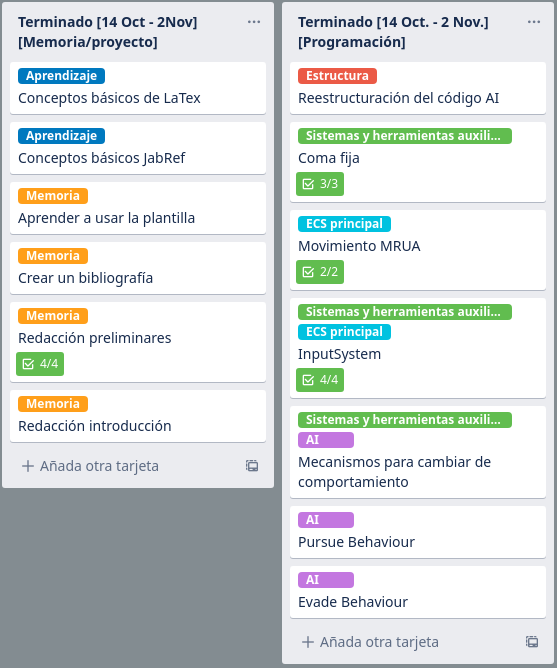
\includegraphics[width=0.45\textwidth]{imagenes/metodologia/tareas_it1.png}
\caption{Lista de tareas realizadas en la iteración 1}
\label{img:it_1}
\end{figure}

\subsection{Iteración 2}
Durante esta tercera iteración los objetivos eran los de corregir el funcionamiento de los
\textit{`Steering behaviors'}, añadir elementos visuales que ayuden al debug de la \ac{IA}
mostrando las componentes del movimiento de las entidades y herramientas para el control del
tiempo de ejecución y el tamaño del \textit{`DeltaTime'}.

Como podemos apreciar en la lista~\ref{img:it_2}, las tareas de control de la ejecución del
programa no fueron realizadas a tiempo, en su lugar se le dió prioridad a mejorar el uso
de la coma fija para un código más limpio y crear metodos auxiliares como puede ser el paso de
coordenadas continuas a pixeles en pantalla, permitiendo así trabajar a lo largo del programa 
usando enteros con signo y procesarlos en el sistema de \textit{`Render'}.

En lo referente a la memoria comenzamos la redacción de una versión preliminar del \ac{GDD},
Estado del Arte y metodología. 

\begin{figure}[ht]
\centering
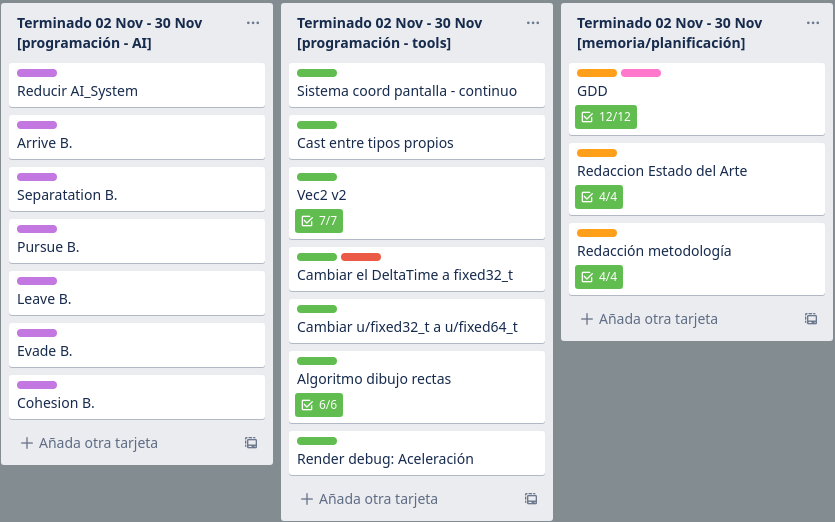
\includegraphics[width=0.65\textwidth]{imagenes/metodologia/tareas_it2.png}
\caption{Lista de tareas realizadas en la iteración 2}
\label{img:it_2}
\end{figure}

